\documentclass[titlepage,landscape]{seminar}
\usepackage{url}
\usepackage{graphicx}
\usepackage[pdftex]{color}
\usepackage{hyperref}
\usepackage{epstopdf}
\usepackage{slides}

\begin{document}

\myslide{
\begin{eqnarray*}
\pi_t &=& \sum_{ij} x_{i\cdot}x_{j\cdot} \delta_{ij} \\
\pi_s &=& \frac{1}{K}\sum_{k=1}^K\sum_{ij} x_{ik}x_{jk}\delta_{ij} \\
\Phi_{st} &=& \frac{\pi_t - \pi_s}{\pi_t}
\end{eqnarray*}
}

\myslide{
\begin{center}
\resizebox{!}{6cm}{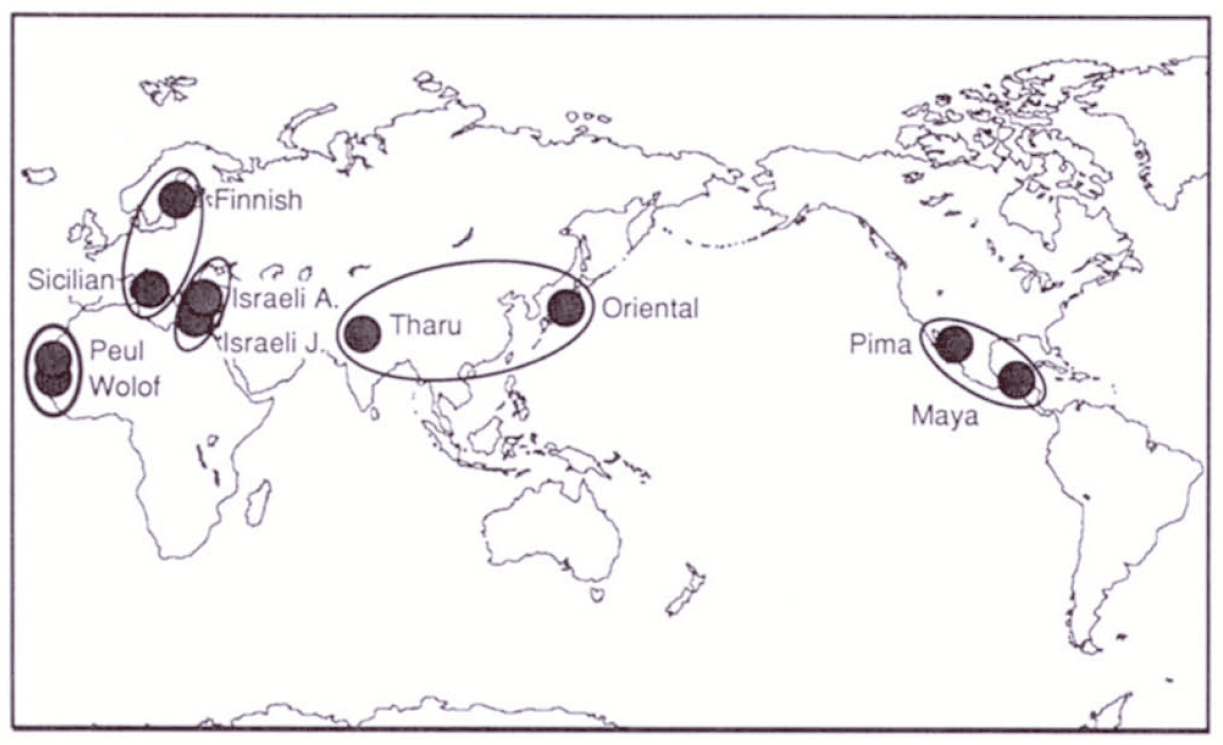
\includegraphics{amova-sample-locations.eps}}
\end{center}
}

\myslide{
\begin{center}
\resizebox{!}{6cm}{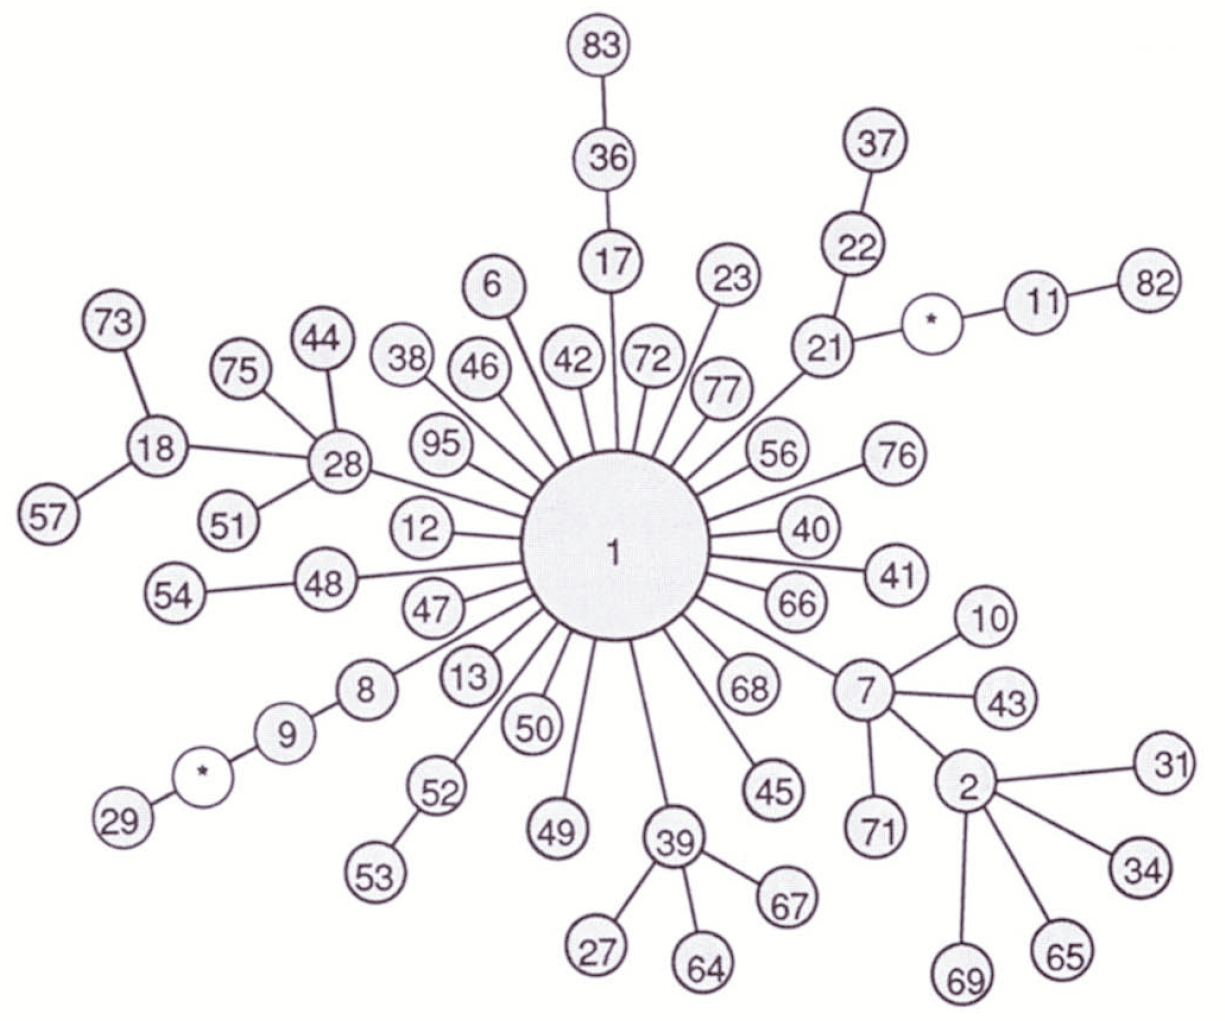
\includegraphics{amova-haplotypes.eps}}
\end{center}
}

\myslide{
\begin{center}
\begin{tabular}{lc}
\hline\hline
Component of differentiation     & $\Phi$-statistics \\
\hline
Among regions                    & $\Phi_{CT} = 0.220$ \\
Among populations within regions & $\Phi_{SC} = 0.044$ \\
Among all populations            & $\Phi_{ST} = 0.246$ \\
\hline
\end{tabular}
\end{center}
}

\myslide{
{\footnotesize
\begin{eqnarray*}
K &=& \mbox{number of populations} \\
P(\mbox{no coalescent}|n, N_e, K) &=& \left(1-\frac{n(n-1)}{4N_e}\right)^K \\
P(\mbox{no migration}|m, K) &=& (1-m)^{nK} \\
P(\mbox{event}|n, m, N_e, K) &=& 1 - P(\mbox{no coalescent}|n, N_e,
K)P(\mbox{no migration}|m, K) \\
P(\mbox{event at }t|n, m, N_e, K) &=& P(\mbox{event}|n, m, N_e,
K)\left(1 - P(\mbox{event}|n, m, N_e, K)\right)^{t-1} \\
\end{eqnarray*}
}
\vfil
\[
P(\mbox{data}|m, N_e) \propto f(n, m, N_e, K)
\]
}

\myslide{
\begin{center}
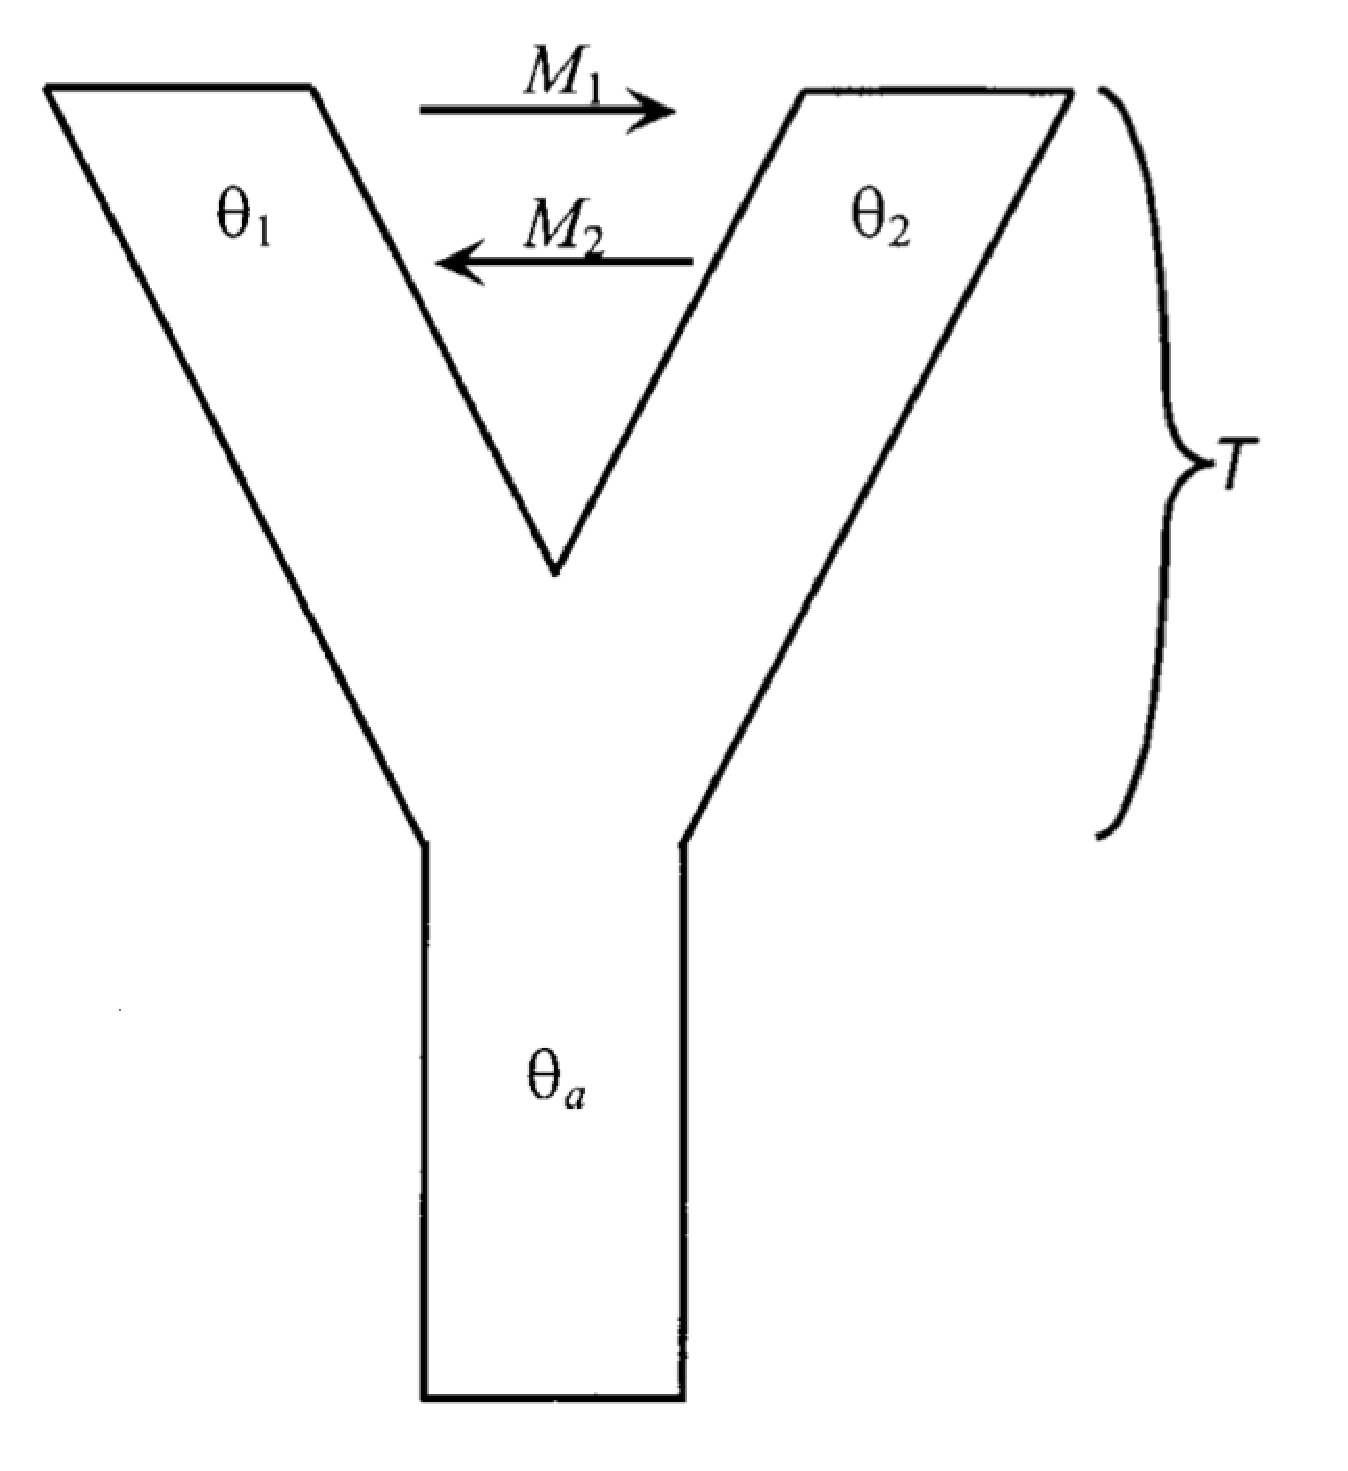
\includegraphics[height=6cm]{nielsen-wakeley.eps}
\end{center}
}

\myslide{
\begin{center}
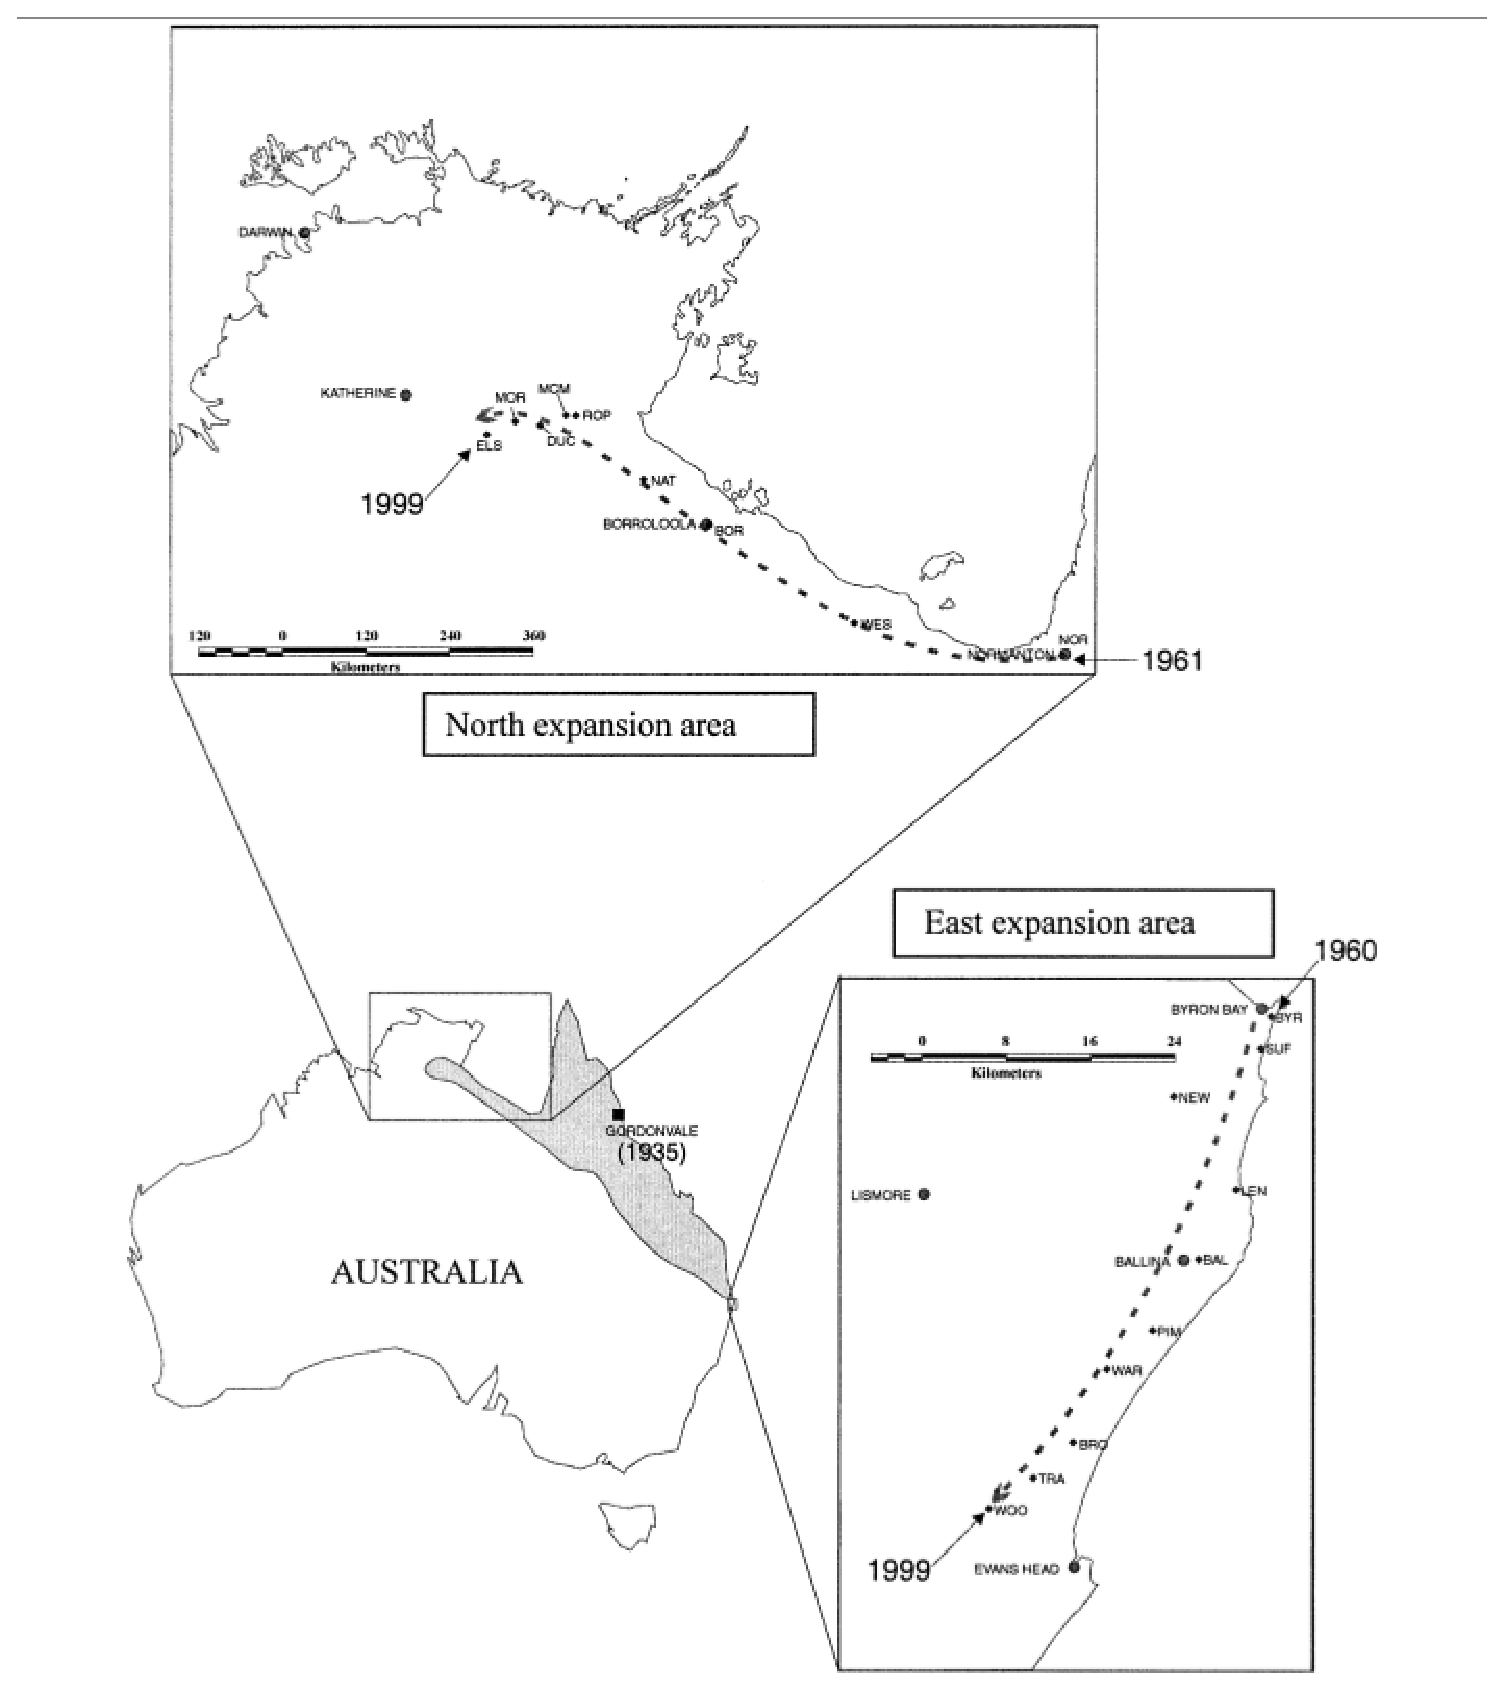
\includegraphics[height=\textheight]{cane-toad-expansion.eps}
\end{center}
}

\myslide{
\begin{center}
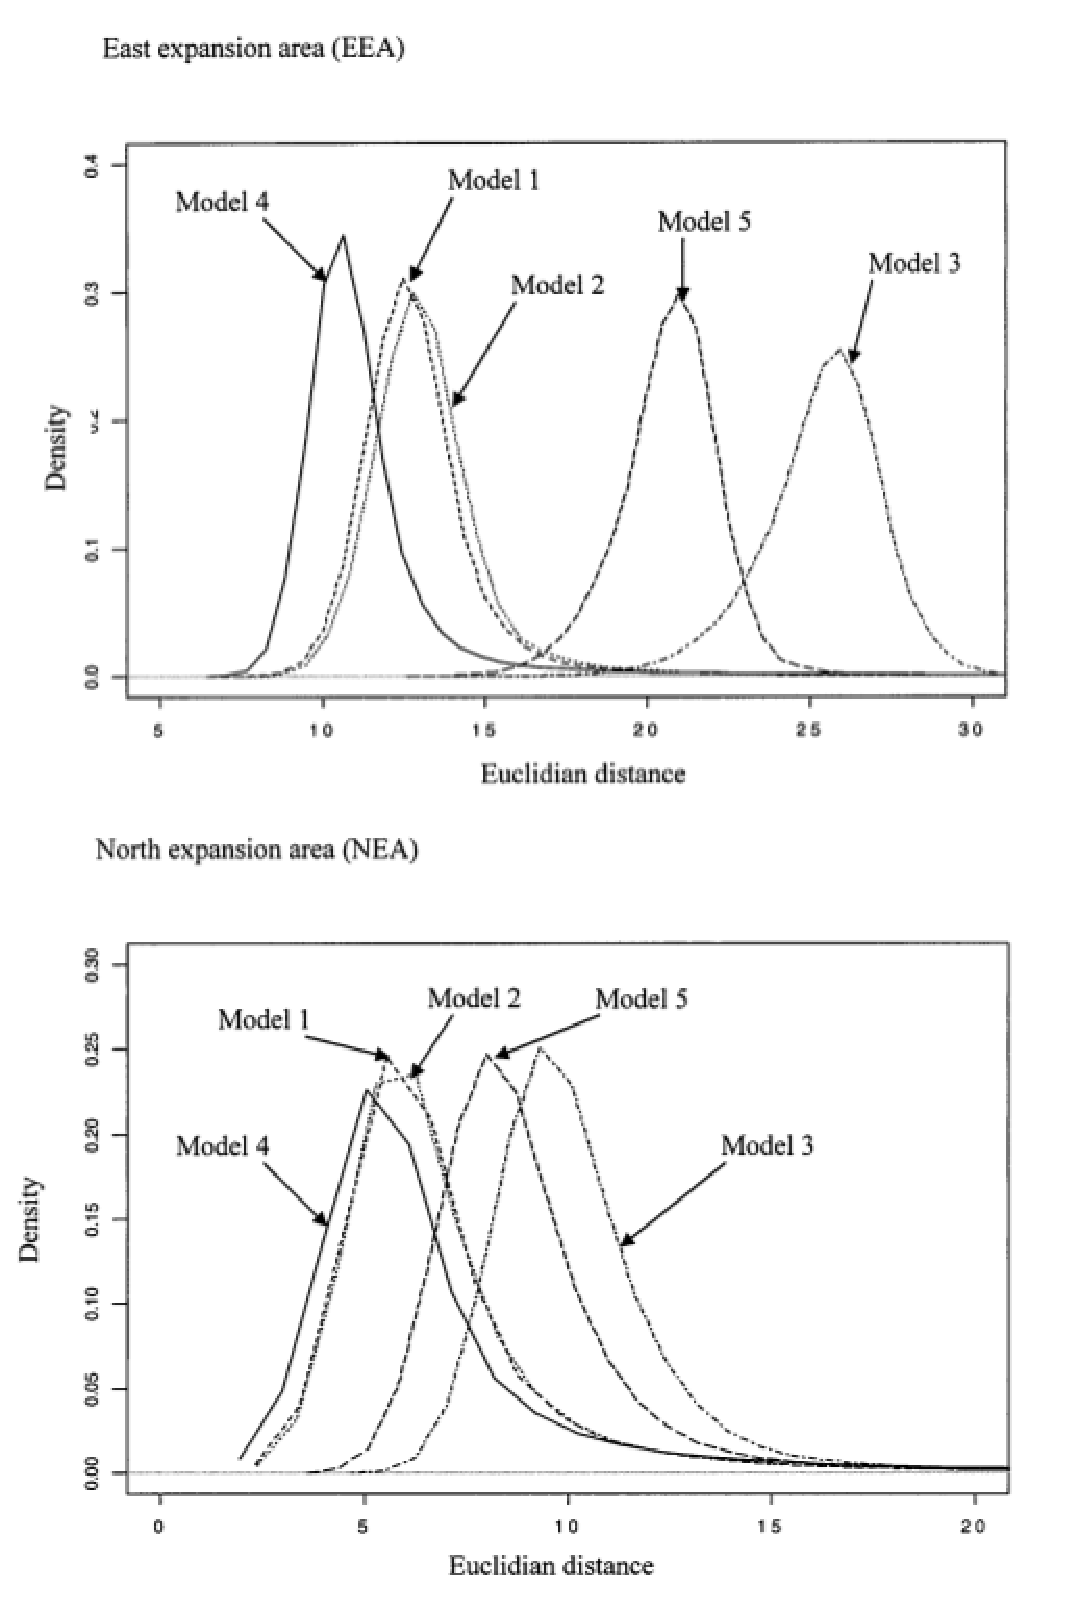
\includegraphics[height=\textheight]{cane-toad-models.eps}
\end{center}
}

\myslide{
\begin{center}
\begin{tabular}{ccr}
\hline\hline
Parameter & area & mean (5\%, 90\%) \\
\hline
$N_{e_s}$ & east & 744 (205, 1442) \\
         & north & 1685 (526, 2838) \\
$N_{e_f}$ & east & 78 (48, 118) \\
         & north & 311 (182, 448) \\
$F_R$    & east & 10.7 (2.4, 23.8) \\
         & north & 5.9 (1.6, 11.8) \\
$m$      & east & 0.014 ($6.0 \times 10^{-6}$, 0.064) \\
         & north & 0.117 ($1.4 \times 10^{-4}$, 0.664) \\
$N_{e_s}m$ & east & 4.7 (0.005, 19.9) \\
          & north & 188 (0.023, 883) \\
\hline
\end{tabular}
\end{center}
}

\end{document}

